\chapter{Proposta}
\label{cap:project}

\begin{quotation}[]{Yoko Ono}
The computer is my favourite invention. I feel lucky to be part of the global village. I don't mean to brag, but I'm so fast with technology. People think it all seems too much, but we'll get used to it. I'm sure it all seemed too much when we were learning to walk.
\end{quotation}

\section{Introdução}
Com o objetivo de facilitar o acesso de usuários à perguntas relacionadas à seu problema, este trabalho traz como proposta um buscador para fóruns de perguntas e respostas. Usaremos apenas o conteúdo e os metadados de uma pergunta para verificar se a mesma pode sanar a dúvida do usuário sendo expressa por uma busca.
\section{Arquitetura}
% Todo usar figuras genéricas
%TODO Migração puxar de base de dados e envia para engenho de busca.
\begin{figure}[htb]
	\centering
	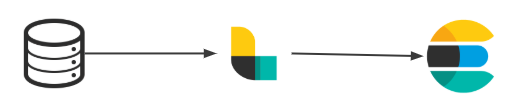
\includegraphics[width=\textwidth]{chapters/project/architecture.png}
	\caption{Arquitetura do sistema proposto}
\end{figure}
Neste projeto, será considerada uma arquitetura plugável à uma base pré-existente, a fim de manter a implantação do sistema o mais simples possível para que outros também possam o implementar em seus fóruns pré-existentes. 
A partir da base já existente do fórum, deve-se ter um serviço que trabalhe de forma contínua extraindo os dados e populando o engenho de busca com estas questões. O pré-processamento pode ser realizado tanto no serviço de migração ou no próprio engenho de busca. Entretanto, é essencial que o engenho de busca seja capaz de indexar e recuperar os dados armazenado de forma eficiente, conforme descrito nesse capítulo.

\section{Modelo Entidade Relacionamento}
\label{mer}

\begin{figure}[htb]
	\centering
	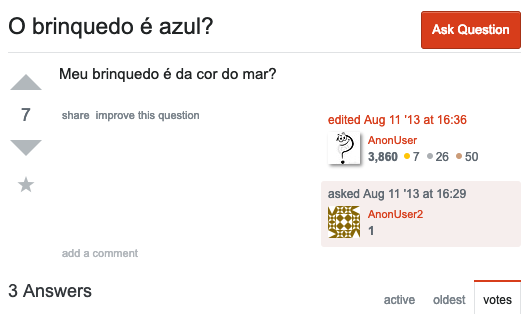
\includegraphics[width=\textwidth]{chapters/project/question-brinquedo.png}
	\caption{Exemplo de questão}
	\label{fig:screenshootquestion}
	% TODO Verificar referências ao AskUbuntu
\end{figure}
Embora nomes, implementações e recursos possam variar de acordo com cada fórum, os fóruns podem ter sua forma adaptada às estruturas descritas nesta seção. 

É conhecido como corpo, o conteúdo textual descritivo em cada uma das perguntas. Nos fóruns observados, foi percebido que as perguntas podem ter tanto título e corpo. Em alguns fóruns, títulos de perguntas podem ser chamados de tópicos, sua primeira mensagem como corpo da pergunta e as mensagens subsequentes como respostas.

Ao permitir que usuários votem indicado a utilidade ou qualidade de um documento, adicionamos um conceito de pontuação. Fóruns que não implementam recursos de avaliação, podem considerar que todos os documentos possuem o mesmo peso ou usar outros parâmetros para definir a pontuação de um documento, como número de visualizações, por exemplo.

\begin{figure}[htb]
	\centering
	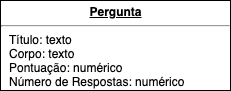
\includegraphics[scale=1.0]{chapters/project/mer.png}
	\caption{Formato da questão exigido}
\end{figure}

\section{Pré-processamento}
Cada pergunta passará por transformações antes de serem armazenadas. Considere os títulos de questões descritas na tabela \ref{tab:example} no seu estado inicial. Estas questões irão ilustrar o pré-processamento. Vale ressaltar que o mesmo processo que está sendo descrito com os títulos também ocorre com o corpo das perguntas.

\begin{table}[htb]
	\centering
    \def\arraystretch{1.2} % padding da linhas da tabela
    \begin{tabular}{|l|l|}
        \hline
        1 & <p>I will organize this room</p>            \\ \hline
        2 & All rooms are organized and clean \\ \hline
        3 & Cleaners are <b>very</b> effective                              \\ \hline
        4 & I will open this window                              \\ \hline
    \end{tabular}
	\caption{Frases de exemplo}
    \label{tab:example}
\end{table}


\subsection{Filtros de caracteres}
Na web é comum encontrar documentos com tags html. Para este projeto, estas tags não terão importância, portanto vamos as remover e deixar apenas o texto.

Após determinar esses filtros, é possível verificar o resultado de alguns exemplos na tabela \ref{tab:charfilter}.

\begin{table}[htb]
	\centering
    \def\arraystretch{1.2} % padding da linhas da tabela
    \begin{tabular}{|l|l|l|}
        \hline
        & \textbf{Antes} & \textbf{Depois} \\ \hline
        1 & <p>I will organize this room</p> & I will organize this room            \\ \hline
        2 & All rooms are organized and clean & All rooms are organized and clean \\ \hline
        3 & Cleaners are <b>very</b> effective & Cleaners are very effective                              \\ \hline
        4 & I will open this window & I will open this window                             \\ \hline
    \end{tabular}
	\caption{Frases de exemplo após os filtros de caracteres}
    \label{tab:charfilter}
\end{table}

\subsection{Tokenização}
O processo de tokenização é responsável por dividir um texto em unidades menores. Essas unidades podem ser palavras, caracteres, cadeia de palavras ou cadeia de caracteres. 

Para este projeto, foi usado a tokenização dividindo o conteúdo do texto em palavras usando o algoritmo Unicode Text Segmentation \cite{unicodesegmentation}.

\begin{table}[htb]
	\centering
    \def\arraystretch{1.2} % padding da linhas da tabela
    \begin{tabular}{|l|l|l|}
        \hline
        & \textbf{Antes} & \textbf{Depois} \\ \hline
        1 & I will organize this room & [I, will, organize, this, room]            \\ \hline
        2 & All rooms are organized and clean & [All, rooms, are, organized, and, clean] \\ \hline
        3 & Cleaners are very effective & [Cleaners, are, very, effective]                              \\ \hline
        4 & I will open this window & [I, will, open, this, window]                             \\ \hline
    \end{tabular}
	\caption{Frases de exemplo após a tokenização}
    \label{tab:tokenization}
\end{table}

\subsection{Transformações}
Algumas transformações podem se fazer necessárias no corpus. Foi usada nesse projeto uma transformação responsável por deixar todos os caracteres minúsculos.

\begin{table}[htb]
	\centering
    \def\arraystretch{1.2} % padding da linhas da tabela
    \begin{tabular}{|l|l|l|}
        \hline
        & \textbf{Antes} & \textbf{Depois} \\ \hline
        1 & [I, will, organize, this, room] & [i, will, organize, this, room]            \\ \hline
        2 & [All, rooms, are, organized, and, clean] & [all, rooms, are, organized, and, clean] \\ \hline
        3 & [Cleaners, are, very, effective] & [cleaners, are, very, effective]                              \\ \hline
        4 & [I, will, open, this, window] & [i, will, open, this, window]                             \\ \hline
    \end{tabular}
	\caption{Frases de exemplo após as transformações}
    \label{tab:transformations}
\end{table}

\subsection{Filtros de tokens}
Existem palavras que adicionam pouco valor semântico ao texto, são conhecidas como \textit{stop words}. Stop words são palavras como: isso, um, a, o, que. Estas também serão removidas. Existem diversas formas de as detectar em um corpus, as mais comuns são com uso de listas com stop words predefinidas ou definindo um limiar máximo de ocorrências que uma palavra pode ter. Assume-se que palavras que ocorrem frequentemente em vários documentos não agregam muito conteúdo ao texto.

\begin{table}[htb]
	\centering
    \def\arraystretch{1.2} % padding da linhas da tabela
    \begin{tabular}{|l|l|l|}
        \hline
        & \textbf{Antes} & \textbf{Depois} \\ \hline
        1 & [i, will, organize, this, room] & [organize, room]            \\ \hline
        2 & [all, rooms, are, organized, and, clean] & [rooms, organized, clean] \\ \hline
        3 & [cleaners, are, very, effective] & [cleaners, effective]                              \\ \hline
        4 & [i, will, open, this, window] & [open, window]                             \\ \hline
    \end{tabular}
	\caption{Frases de exemplo após os filtros de tokens}
    \label{tab:tokenfilter}
\end{table}

\subsection{Stemming}
O propósito do stemming é reduzir a variação morfológica das palavras \cite{stemmingdef}. Documentos podem usar formas diferentes de uma palavra, por exemplo, um deles pode usar organizar, outro pode usar organizando e outro organizado. Embora as palavras não sejam idênticas, elas trazem consigo um sentido similar, o que pode ser útil em um sistema de recuperação da informação onde se deseja conteúdo relacionado, ainda que não idêntico.

\begin{figure}[htb]
	\centering
	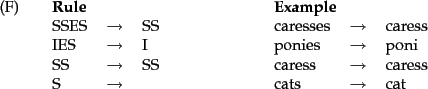
\includegraphics[width=\textwidth]{chapters/project/porterrules.png}
	\caption{Regras usadas na primeira fase do Porter Stemmer}
    \label{fig:porterstemmerprocess}
\end{figure}

O algoritmo mais comum de Stemming é o Porter \cite{porterstemming}. Este algoritmo usa fases com conjuntos definidos de regras para definir as transformações que uma dada palavra irá passar. A figura \ref{fig:porterstemmerprocess} mostra algumas das regras executadas na primeira fase do algoritmo.

Percebe-se que agora, que as frases descritas na tabela x, possuem mais palavras em comum do que anteriormente, isso garante uma busca mais abrangente, permitindo o usuário ter resultados com palavras diferentes da sua, mas que ainda acessem o mesmo domínio.
%TODO Inserir conjunto de frases diferentes antes do stemming que ficam mais parecidas após o stemmin

\begin{table}[htb]
	\centering
    \def\arraystretch{1.2} % padding da linhas da tabela
    \begin{tabular}{|l|l|l|}
        \hline
        & \textbf{Antes} & \textbf{Depois} \\ \hline
        1 & [organize, room]  & [organ, room]            \\ \hline
        2 & [rooms, organized, clean]  & [room, organ, clean] \\ \hline
        3 & [cleaners, effective]  & [cleaner, effect]                              \\ \hline
        4 & [open, window]  & [open, window]                             \\ \hline
    \end{tabular}
	\caption{Frases de exemplo após os filtros de tokens}
    \label{tab:tokenfilter}
\end{table}

\subsection{Sumário}
Percebe-se na tabela \ref{tab:allphrases} o quanto cada uma das frases mudou e agora é possível verificar alguns padrões se repetindo onde não seria tão fácil se identificar previamente.
\begin{table}[htb]
	\centering
    \def\arraystretch{1.2} % padding da linhas da tabela
    \begin{tabular}{|l|l|l|}
        \hline
        & \textbf{Incial} & \textbf{Final} \\ \hline
        1 & <p>I will organize this room</p>  & [organ, room]            \\ \hline
        2 & All rooms are organized and clean  & [room, organ, clean] \\ \hline
        3 & Cleaners are <b>very</b> effective  & [cleaner, effect]                              \\ \hline
        4 & I will open this window  & [open, window]                             \\ \hline
    \end{tabular}
	\caption{Frases de exemplo após o pré-processamento}
    \label{tab:allphrases}
\end{table}

 Na tabela \ref{tab:quenstionpreprocessed} percebe-se o mesmo processo aplicado aos campos título e corpo de uma pergunta.

\begin{table}[htb]
	\centering
    \def\arraystretch{1.2} % padding da linhas da tabela
    \begin{tabular}{|l|l|l|}
        \hline
        & \textbf{Inicial} & \textbf{Final} \\ \hline
        \textbf{Título}              & O brinquedo é azul?            & [brinq, azul] \\ \hline
        \textbf{Corpo}               & Meu brinquedo é da cor do mar? & [brinq, cor, mar] \\ \hline
        \textbf{Pontuação}           & 7                              & 7 \\ \hline
        \textbf{Número de respostas} & 3                              & 3 \\ \hline
    \end{tabular}
	\caption{Questão após o pré-processamento}
    \label{tab:quenstionpreprocessed}
\end{table}     

\section{Indexação e Recuperação}
Concluído o pré-processamento, deve-se armazenar estes documentos, de forma que seja possível os recuperar em outro momento. Entretanto, métodos comuns encontrados na maioria dos bancos de dados são inadequados para lidar com texto.

Índices invertidos foram criados para serem uma forma rápida para lidar com dados massivos de texto. Para cada termo, é salvo o número de ocorrências e em que documentos eles ocorrem, conforme descrito na tabela \ref{tab:invertedindex}. Para cada campo de uma pergunta, existe um índice, ou seja, além do índice dos títulos na tabela \ref{tab:invertedindex}, ao realizar o pré-processamento do corpo das perguntas, também haverá um índice para os corpos.

\begin{table}[htb]
	\centering
    \def\arraystretch{1.2} 
    \begin{tabular}{|l|l|l|}
        \hline
        \textbf{Termo} & \textbf{Frequência} & \textbf{Documentos} \\ \hline
        organ & 2  & 1, 2            \\ \hline
        room & 1  & 2 \\ \hline
        clean & 1  & 2                              \\ \hline
        cleaner & 1  & 3                             \\ \hline
        effect & 1  & 3                             \\ \hline
        open & 1  & 4                             \\ \hline
        window & 1  & 4                             \\ \hline
    \end{tabular}
	\caption{Frases de exemplo no índice invertido}
    \label{tab:invertedindex}
\end{table}

Ao executar uma busca, o texto informado pelo usuário passa pelo mesmo processo de preprocessamento que as questões passaram. Dessa forma, os tokens gerados ao final do pré-processamento serão usados para encontrar questões já existentes na base que possuam um ou mais tokens em comum. 

\section{Ranking}
Na seção anterior, foi explicado como encontrar documentos relacionados. Nesta seção será explicado como definir a prioridade entre os selecionados, ou seja, determinar quais devem aparecer primeiro.

\subsection{Cálculo de Similaridade}
Conforme descrito no capítulo \ref{cap:informationretrieval}, pode-se usar o \ac{TFIDF} para verificar o grau de importância de um termo e a similaridade do cosseno para comparar a similaridade de dois documentos.

\begin{table}[htb]
	\centering
    \def\arraystretch{1.2}
    \begin{tabular}{|l|l|l|l|l|l|l|l|l|}
        \hline
        Questão & organ & room & clean & cleaner & effect & open & window & \textbf{Sim. busca}\\ \hline
        1 & 0 & 0 & 0 & 0 & 0 & 0 & 0 & 0 \\ \hline
        2 & 0 & 0 & 0 & 0 & 0 & 0 & 0 & 0 \\ \hline
        3 & 0 & 0 & 0 & 0 & 0 & 0 & 0 & 0 \\ \hline
        4 & 0 & 0 & 0 & 0 & 0 & 0 & 0 & 0 \\ \hline
    \end{tabular}
	\caption{TFIDF e a similaridade com a busca das frases de exemplo}
    \label{tab:tfidf}
\end{table}

A partir dessas informações, já é possível ordenar os resultados com base no valor de similaridade, onde quanto maior este número, melhor sua posição no ranking. 

%TODO Comentar resultados

\subsection{Cálculo de Relevância}
Desde a seção anterior já é possível recuperar perguntas semelhantes à busca feita pelo usuário, mas ainda não se é verificada a relevância que as mesmas têm. Uma pergunta que possua a mesma intenção que a da busca realizada, não, necessariamente, terá um conteúdo relevante. Para resolver problema, é necessário verificar, dentre as semelhantes, quais são melhor reconhecidas pela comunidade como mais úteis.

Na tabela \ref{tab:relevance} é exemplificado o cálculo de relevância com as frases de exemplo. Para o campo da similaridade com o título, o valor usado será o mesmo dos exemplos anteriores. No campo de similaridade com o corpo, o mesmo processo que ocorreu com o título é usado para calcular o deste. Serão introduzidos valores fictícios para o valor da pontuação.

\begin{table}[htb]
	\centering
    \def\arraystretch{1.2} % padding da linhas da tabela
    \begin{tabular}{|l|l|l|l|l|}
        \hline
        Questão & Sim. título & Sim. corpo & Pontuação & \textbf{Relevância} \\ \hline
        1 & 0 & 0 & 7 & 0 \\ \hline
        2 & 0 & 0 & 2 & 0 \\ \hline
        3 & 0 & 0 & 1000 & 0 \\ \hline
        4 & 0 & 0 & 1 & 0 \\ \hline
    \end{tabular}
	\caption{Cálculo de relevância das frases de exemplo}
    \label{tab:relevance}
\end{table}

A equação \ref{eq:rel} foi utilizada para fazer o cálculo da relevância. A função \textit{sim} é responsável por calcular a similaridade entre dois textos. A variável \textit{q} é uma questão indexada no engenho de busca.
%Explicar razões da equação ser como é
%TODO Comentar resultados
\begin{equation}
    Rel(q, busca) = sim(Titulo_{q}, busca) sim(Corpo_{q}, busca) Pontuacao_{q} 
    \label{eq:rel}
\end{equation}

\section{Tecnologias Utilizadas}
Para tornar essa aplicação real, foi usado um conjunto de ferramentas que auxiliam os processos descritos anteriormente nesse capítulo.
\begin{itemize}
    \item ElasticSearch
    \item Logstash
    \item Kibana
    \item MySQL
    \item Docker
    \item Python
\end{itemize}
\section{Sumário}
